\section{Dataset and Experiment Design}
\subsection{Piggyback}
\subsubsection{Theorem}
\begin{figure}
  \centering
  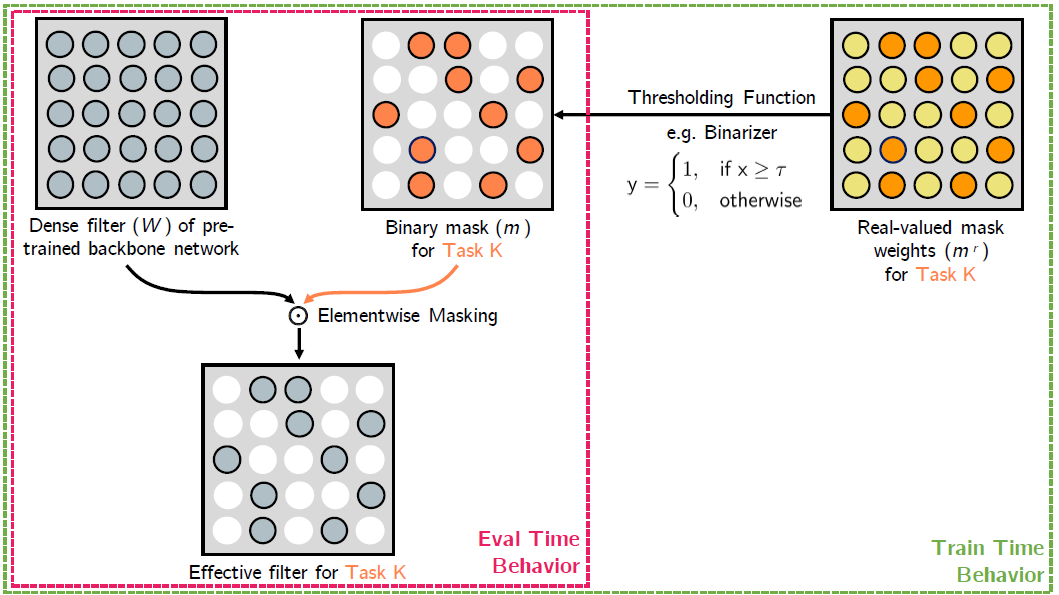
\includegraphics[width=0.8\textwidth]{figure/piggyback.png}
  \caption{Piggyback Overview}
  \label{piggy}
\end{figure}

Piggyback adopts masking weight for new task to overcome catastrophic forgetting. The core idea is to selectively mask the fixed weights of a base network, and then use this mask to predict the new task. That is, given model $\mathbf{W}$, the optimizer will genrate and optimize a binary mask weight $\mathbf{W}^\star$. The gradient that backpropagates to the layer will not affect $\mathbf{W}$ but $\mathbf{W}^{\star}$. In this way, for a given task, we can obtain a filter vecotor that is consist of 0/1. For example, a weight dense vector [0.1, 0.2, 0.3, 0.4] can be filtered to [0, 0.2, 0.3, 0] after the binary masking. In short, we does not learn what are the `right` parameters but learn what is not the `right` parameters. Therefore, the choice of backbone network is crucial to the performance of piggyback because if the original weights are malfunctioning, pure masking cannot greatly improve the accuracy.

The structure of \textit{Piggyback} is shown in figure \ref{piggy}. To explain the procedure for training, we consider an end to end fully-connected layer case. Denote $\mathbf{x}=[x_1, x_2, ..., x_m]$ as input, and $\mathbf{y}=[y_1, y_2, ..., y_n]$ as output. Therefore the weight matrix is $\mathbf{W}^{n\times m}$. Without loss of genrality, we can simply assume $\mathbf{y}=\mathbf{W}\mathbf{x}$ by ignoring the bias term. Suppose the loss function is $L$, the backpropagation equation for $\mathbf{W}$ is,
\begin{equation}
\centering
\begin{aligned}
\delta w_{ji}&=\frac{\partial L}{\partial w_{ji}} = (\frac{\partial L}{\partial y_j})\cdot (\frac{\partial y_j}{\partial w_{ji}}) \\
&= \delta y_j \cdot x_j \\
\therefore \delta \mathbf{W} &= \delta \mathbf{y} \cdot  \mathbf{x^T} \\
\end{aligned}
\end{equation}
In \textit{Piggyback}, the author has introduced a real value matrix $\mathbf{M_r}^{n\times m}$ and a manually set threshold $\tau$. We denote the mask matrices as $\mathbf{M}=[m]_{ji}$, and we can obtain $m_{ji}$ by,
\begin{equation}
m_{ji}=\begin{cases}
1,\ \ &{\rm if}\ m^r_{ji}>\tau \\
0,\ \ &{\rm otherwise} \\
\end{cases}
\end{equation}
Then, for $y_j\in\mathbf{y}$, it gives $y_j=\sum_{i=1}^m w_{ji}\cdot m_{ji} \cdot x_i$. The backpropagation equation is used to update the real value matrix $M_r$. That is, during the whole training procedure, the weight matrix $\mathbf{W}$ is fixed as constant. In \textit{Piggyback}, the mask weigths updates as follows. Here, $A\odot B = C=[c_{ji}=A_{ji}B_{ji}]$. 

\begin{equation}
\begin{aligned}
\delta m_{ji}=\frac{\partial L}{\partial m_{ji}} &= (\frac{\partial L}{\partial y_j})\cdot (\frac{\partial y_j}{\partial m_{ji}}) \\
&= \delta y_j \cdot w_{ji} \cdot x_j \\
\therefore \delta \mathbf{m} &= (\delta \mathbf{y} \cdot x^T) \odot \mathbf{W} \\
\end{aligned}
\end{equation}
\subsubsection{Experiment Setting}
In practical, it is hard to derive the analytical solution to threshold $\tau$. In the original work, the author set $\tau=5e-3$. As for the matrix $\mathbf{m_r}$, the author initialized the value to 0.01. The best results are produced by Adam optimizer. In our experiment, we have inherited the parameter settings in the work. However, as mentioned in the previous statement, the crucial part for \textit{Piggyback} is that the base model have to be fine-tuned, otherwise the model will not work very well. We have also verified such phenomon in our experiment. To improve the performance, we modified the logic of the model. At the first task, we use the pure base model to perform the training, as the pre-trained network(ResNet50\cite{he2016deep}, in our case)cannot perform well on the given dataset. Then we begin performing mask and \textit{Piggyback}. This part will later be discussed in detail in Section \ref{eval}.





